
\chapter{Code MDFT\label{chpt:mdft}}

The code MDFT upon which all the development in this thesis is
based is a Fortran 95 sequential code developed by Maximilien Levesque,
Daniel Borgis \textit{et al.} \citep{gendre_classical_2009,jeanmairet_molecular_2013-1,jeanmairet_molecular_2015,jeanmairet_molecular_2016,Jeanmairet_thesis,levesque_solvation_2012,ramirez_density_2002,ramirez_density_2005,sergiievskyi_fast_2014,Zhao_2011},
which implements the \acs{MDFT} theory. It reads the force field (Lennard-Jones
and Coulomb parameters) describing the solute and the solvent as input,
as well as necessary parameters like the temperature $T$, number
density of solvent $n_{0}$, etc. It minimizes the functional and
gives the equilibrium density $\rho(\mathbf{r},\mathbf{\Omega})$,
then computes output properties.

\section{Supercell discretization}

$L_{x}\times L_{y}\times L_{z}$ $\left[\textrm{Å}^{3}\right]$ space
is discretized on a regular grid of $\textrm{nfft}_{1}\times\textrm{nfft}_{2}\times\textrm{nfft}_{3}$
nodes. The solute center is at $\mathbf{r}_{T}=\left(\dfrac{L_{x}}{2},\dfrac{L_{y}}{2},\dfrac{L_{z}}{2}\right)$
of the box. If the internal coordinates of solute $\mathbf{r}_{M}$,
the solute coordinates in the box $\mathbf{r}=\mathbf{r}_{M}+\mathbf{r}_{T}$.

Angular grid is discretized with Lebedev (L) quadrature for $\mathbf{\Omega}\equiv\left(\Theta,\Phi\right)$,
$\Theta\in\left[0,\pi\right]$, $\Phi\in\left[0,2\pi\right]$, or
Gauss-Legendre (GL) quadrature for $\Theta$ and trapezoidal quadrature
for $\Phi$. $\Psi\in\left[0,\pi\right]$ as we used the code mainly
for water, is discretized with trapezoidal quadrature. The number
of each angular dimension is linked to the order of quadrature, $m_{\max}$,
which is discussed mainly in the chapter of theory.

\section{Minimizer L-BFGS-B}

The minimizer adopted by \acs{MDFT} is the L-BFGS-B \citep{Zhu_1994_bfgs,Zhu_bfgs_1997_algorithm}
package version 3.0 written in Fortran 77, implementing the limited-memory
Broyden-Fletcher-Goldfarb-Shanno (BFGS) algorithm with constraints
of the form $l\leq x\leq u$ to the variable $x$.

The functional $\mathcal{F}[x_{i}]$ and the gradient of functional
$\nabla\mathcal{F}[x_{i}]=\dfrac{\delta\mathcal{F}}{\delta x}(x_{i})$
are required by L-BFGS to minimize the functional. It saves the variables
$x_{i}$ and gradients of the past $m$ iterations, which requires
a lot of memory.

The functional in MDFT to be minimized is eq. (\ref{eq:4.fff}):
\begin{equation}
\mathcal{F}[\rho]=\mathcal{F}_{\mathrm{id}}[\rho]+\mathcal{F}_{\mathrm{ext}}[\rho]+\mathcal{F}_{\mathrm{exc}}[\rho]
\end{equation}
and its gradient is
\begin{equation}
\frac{\delta\mathcal{F}[\rho]}{\delta\rho(\mathbf{r},\mathbf{\Omega})}=k_{\mathrm{B}}T\ln\left(\dfrac{\rho(\mathbf{r},\mathbf{\Omega})}{\rho_{0}}\right)+V_{\mathrm{exc}}(\mathbf{r},\mathbf{\Omega})+V_{\mathrm{ext}}(\mathbf{r},\mathbf{\Omega})
\end{equation}
where $\rho_{0}$ is the angular density of bulk solvent, 
\begin{equation}
\rho_{0}=\left\{ \begin{array}{ll}
n_{0} & \mbox{if atomic, }\Omega\equiv1\\
n_{0}/4\pi & \mbox{if linear, }\Omega\equiv(\Theta,\Phi)\\
n_{0}/8\pi^{2} & \mbox{if non-linear, }\Omega\equiv(\Theta,\Phi,\Psi)
\end{array}\right.\label{eq:rho}
\end{equation}
such that $\int\mathrm{d}\mathbf{\Omega}\rho(\mathbf{r},\mathbf{\Omega})/\rho_{0}=n(\mathbf{r})/n_{0}$
is normalized to 1 when $r\rightarrow\infty$.

\section{Treatment to avoid unphysical density}

During minimization, the density variable $\rho(\mathbf{r},\mathbf{\Omega})$
can have unphysical negative numbers, which also cause the divergence
of the minimization. To avoid this phenomenon, a normalized $\varphi(\mathbf{r},\mathbf{\Omega})$
is used as the variable during the minimization in place of $\rho(\mathbf{r},\mathbf{\Omega})$,
so that:
\begin{equation}
\rho(\mathbf{r},\mathbf{\Omega})=\rho_{0}\varphi^{2}(\mathbf{r},\mathbf{\Omega})\label{eq:cg_vect}
\end{equation}

According to the definition (\ref{eq:cg_vect}), we see:
\begin{equation}
\frac{\delta\rho(\mathbf{r},\mathbf{\Omega})}{\delta\varphi}=2\rho_{0}\varphi(\mathbf{r},\mathbf{\Omega})
\end{equation}

Therefore the gradient to feed the L-BFGS minimizer is:
\begin{equation}
\frac{\delta\mathcal{F}}{\delta\varphi}=\frac{\delta\mathcal{F}}{\delta\rho}\cdot\frac{\delta\rho}{\delta\varphi}=2\rho_{0}\varphi(\mathbf{r},\mathbf{\Omega})\cdot\left[\beta^{-1}\ln\varphi^{2}+V_{\mathrm{exc}}+V_{\mathrm{ext}}\right]
\end{equation}

The main structure of the code is shown in figure \ref{fig:code-mdft}.
\begin{figure}[H]
\begin{centering}
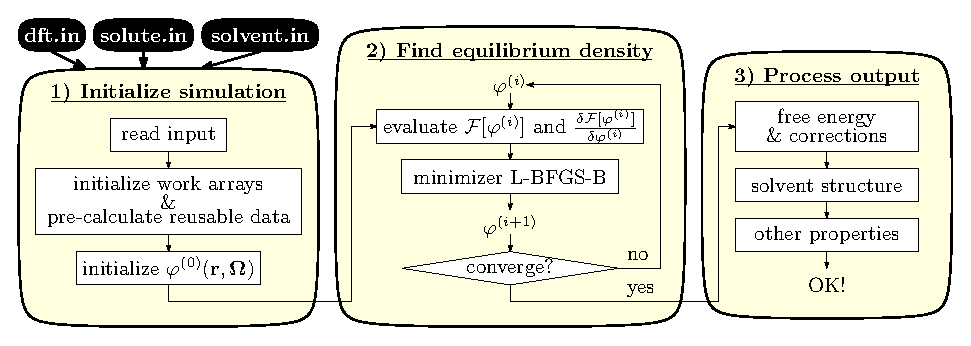
\includegraphics[width=1\columnwidth]{_figure/mdft}
\par\end{centering}
\caption{Main structure of code MDFT\label{fig:code-mdft}}
\end{figure}


\section{Fast Fourier transform}

The fast Fourier transform (\acs{FFT}) is used in the
evaluation of excess functional in eq. (\ref{eq:4.gamma-k}); in this
thesis, the FFTW3 library \citep{FFTW3} is used for implementation,
which performs discrete Fourier Transform (\acs{DFT}) as defined
below:
\begin{equation}
Y_{k}=\sum_{j=0}^{n-1}X_{j}e^{-2\pi ijk/n}\begin{array}{c}
\mathrm{(forward)}\end{array}\label{eq:fftw3-fwd}
\end{equation}
\begin{equation}
X_{j}=\sum_{k=0}^{n-1}Y_{k}e^{2\pi ijk/n}\begin{array}{c}
\mathrm{(backward)}\end{array}\label{eq:fftw3-bwd}
\end{equation}

Note that after a forward-backward Fourier transform, the original
function is multiplied by a normalization factor $N_{k}$, which is
the total number of nodes $k$.

For input function $Y_{k}$ $(k=0,\ldots,n-1)$ in real numbers, FFTW3
only outputs elements $k=0,\ldots,\left\lfloor n/2\right\rfloor $
( $\left\lfloor n/2\right\rfloor +1$ complex numbers of $X_{j}$
are stocked; $\left\lfloor n/2\right\rfloor $ being the floor function
of $n/2$), with the “Hermitian” symmetry
\begin{equation}
Y_{k}=Y_{n-k}^{*}\label{eq:yk_conjg}
\end{equation}
used to regenerate elements of $k>\left\lfloor n/2\right\rfloor $.
The resulting $X_{j}$ issued from the corresponding backward transform
is purely real. 

The definition of \acs{FFT} can differ in some literature, with
the ``$+$'' sign in the exponential of forward transform and ``$-$''
sign in the exponential of backward transform. According to the Hermitian
symmetry, we should use the quantities in $k$-space issued from such
a definition with its conjugate form.
